%*****************************************
\chapter{Regression}\label{reg:regression}
%*****************************************
%TODO Reviewed

\section{Introduction}

Regression is a method used to describe relationships between two variables. Regression is similar to correlation, but it is a measure of the relationship between the \textit{mean} of one variable and the corresponding values of another variable. Regression analysis is used to predict an unknown value for one variable when the mean of the related variable is known. For example, if some research project plotted the ages of people who started smoking and the family income of those people then a correlation would attempt to determine if there is some relationship between those two factors while a regression would attempt to predict the age someone would start smoking given that person's family income.

This lab explores the statistics of regression and demonstrates how to use regression to make predictions.

\section{Regression}

A regression line can be drawn on a scatter plot to graphically show the relationship between two variables (this is sometimes called a ``trend line'' and a ``line of best fit''). Moreover, if the data points in the scatter plot are all close to the regression line, then it is a strong correlation.

As an example, in the \textit{bdims} dataset the calculated Pearson's r for weight and ankle diameter was $ 0.726 $. The regression line in Figure \ref{reg:weight_ankle_diameter} makes it clear that the correlation is positive (the line slopes up and right) and since the dots are all fairly close to the regression line the correlation is strong. 

\begin{figure}[H]
  \begin{center}
    \fbox{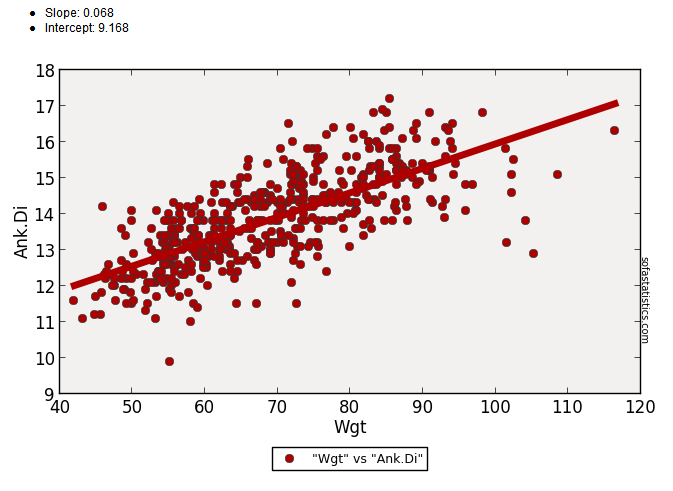
\includegraphics[width=0.95\linewidth]{gfx/reg005}}
    \caption{Weight-Ankle Diameter}
    \label{reg:weight_ankle_diameter}
  \end{center}
\end{figure}

As another scatter plot example, here is one for height and hip girth.

\begin{figure}[H]
  \begin{center}
    \fbox{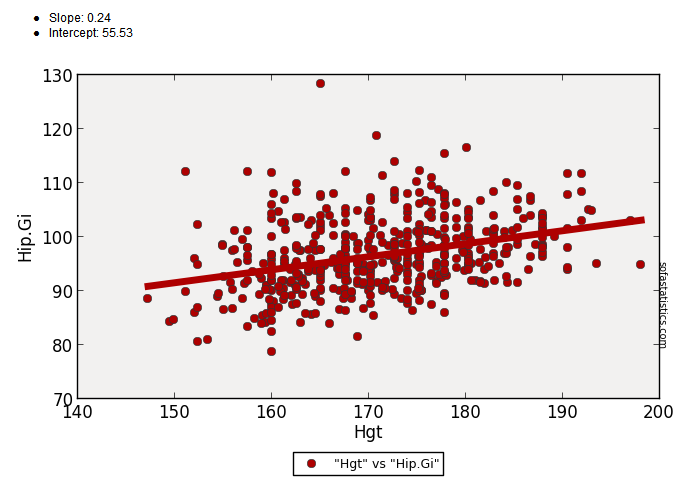
\includegraphics[width=\linewidth]{gfx/reg010}}
    \caption{Height-Hip Girth}
    \label{reg:weight_hip_girth}
  \end{center}
\end{figure}

The correlation for height and hip girth is $ 0.339 $. While this is a positive number, it is weakly positive so the slope of the regression line is small and the dots are fairly scattered.

\texttt{SOFA} includes the slope and Y-Intercept data at the top left corner of a regression plot. That information can be used to predict the Y-Value for a given X-Value by using a simple ``Slope-Intercept'' equation:

\[ y = mx + b \]

Where $ m $ is the slope of the regression line and $ b $ is the y-intercept. By plugging in a value for $ x $ a simple calculation will determine the corresponding value for $ y $. For example, in Figure \ref{reg:weight_hip_girth} the slope is $ 0.241 $ and the y-intercept is $ 55.427 $. To calculate the Hip Girth (the ``y'' value) for a height of $ 165 $ centimeters:

\begin{align}
\notag
  y &= (0.241)(165)+55.427 \\
  \notag
  y &= 95.192
\end{align}

It is important to keep in mind that Pearson's r and the slope of the regression line measure different aspects of a correlation, and even though they could coincidentally be nearly the same they should not be confused. It is possible to have a slope, for example, of $ -2.0 $, but never a correlation that size. In the case of Figure \ref{reg:weight_hip_girth}, the slope is $ 0.241 $ while the correlation is $ 0.339 $.

Regression analysis becomes less certain if the selected X-Value is at the edge or outside the main body of the scatter plot. For example, in Figure \ref{reg:weight_hip_girth} it is mathematically possible to predict the value of hip girth (Y-Value) for a height of $ 140 $ centimeters (X-Value):

\begin{align}
  \notag
  y &= (0.241)(140)+55.427 \\
  \notag
  y &= 89.167
\end{align}

However, since the selected X-Value is outside the main body of the scatter plot then the calculated Y-Value is suspect.

\section{Procedure}

Start \texttt{SOFA} and select ``Statistics'' then:

\begin{enumerate}
  \item Select ``Select a Statistical Test Here''
  \item Select ``Correlation - Pearson's''
  \item Click ``Configure Test''
  \item Data Source Table: gifted (It is desired to predict a child's score on a test of analytical skills when given the mother's IQ.)
  \item Group A: Motheriq (this is the ``X-Axis'' or independent variable)
  \item Group B: Score (this is the ``Y-Axis'' or dependent variable)

  \begin{figure}[H]
    \begin{center}
      \fbox{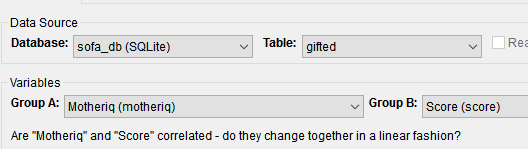
\includegraphics[width=\linewidth]{gfx/reg015}}
      \caption{Calculating Pearson's R for Motheriq-Score}
    \end{center}
  \end{figure}

  \item Click ``Show Results'' and scroll down to the scatter plot.
  
  \begin{figure}[H]
    \begin{center}
      \fbox{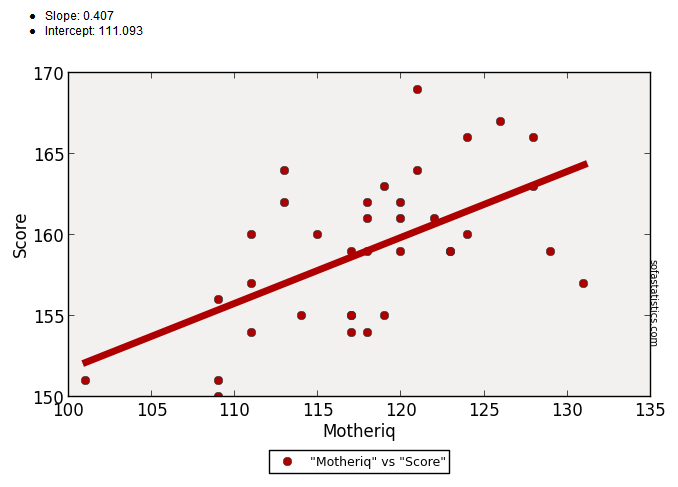
\includegraphics[width=\linewidth]{gfx/reg020}}
      \caption{Scatter Plot for Motheriq-Score}
    \end{center}
  \end{figure}

  \item Using the slope and y-intercept, calculate the expected test score for a mother's IQ of 118.

  \begin{align}
    \notag
    y &= (0.407)(118)+111.093 \\
    \notag
    y &= 159.119
  \end{align}

  \item Using the slope and y-intercept, calculate the expected test score for a mother's IQ of 122.

  \begin{align}
    \notag
    y &= (0.407)(122)+111.093 \\
    \notag
    y &= 160.747
  \end{align}

\end{enumerate}

The following table lists the predicted student's test score for several different variables in the \textit{gifted} dataset. This could be used for practice in calculating regression predictions. In each case, Pearsons r was calculated and the ``Group B'' used is ``Score.''

\rowcolors{1}{gray!25}{}
\begin{center}
  \begin{tabular}{lcccc}
    \hline 
    \textbf{Group A} & \textbf{Slope} & \textbf{Intercept} & \textbf{X-Value} & \textbf{Predicted Score} \\ 
    \hline 
    Fatheriq     & $ 0.25 $ & $ 130.429 $ & $ 117 $ & $ 159.679 $ \\ 
    Read      & $ 11.813 $ & $  133.905 $ & $ 2.35 $ & $ 161.67 $  \\ 
    Speak   & $ 0.385 $ & $ 152.216 $ & $ 17 $ & $ 158.761 $ \\ 
    \hline 
  \end{tabular} 
\end{center}

\subsection{Activity 1: Predictive Regression 1} \label{reg:act01}

Using the \textit{maincafe} dataset in \texttt{SOFA}, determine the slope and intercept for Length (Group A) and Bill (Group B). Use those numbers to predict the bill for a meal lasting $ 42 $ minutes. Round the bill to the nearest penny.

\subsection{Activity 2: Predictive Regression 2} \label{reg:act02}

Using the \textit{maincafe} dataset in \texttt{SOFA}, determine the slope and intercept for Age (Group A) and Tip (Group B). Use those numbers to predict the tip left by a customer who is $ 48 $ years old. Round the tip to the nearest penny.

\section{Deliverable}

Complete the following activities in this lab:

\rowcolors{1}{gray!25}{}
\begin{center}
  \begin{tabular}{lll}
    \hline 
    \textbf{Number} & \textbf{Name} & \textbf{Page} \\ 
    \hline 
    \ref{reg:act01} & \nameref{reg:act01} & \pageref{reg:act01} \\ 
    \ref{reg:act02} & \nameref{reg:act02} & \pageref{reg:act02} \\ 
    \hline 
  \end{tabular} 
\end{center}

Consolidate the responses for all activities into a single document and submit that document for grading.

